
% LaTeX Beamer file automatically generated from DocOnce
% https://github.com/hplgit/doconce

%-------------------- begin beamer-specific preamble ----------------------

\documentclass{beamer}

\usetheme{blue_plain}
\usecolortheme{default}

% turn off the almost invisible, yet disturbing, navigation symbols:
\setbeamertemplate{navigation symbols}{}

% Examples on customization:
%\usecolortheme[named=RawSienna]{structure}
%\usetheme[height=7mm]{Rochester}
%\setbeamerfont{frametitle}{family=\rmfamily,shape=\itshape}
%\setbeamertemplate{items}[ball]
%\setbeamertemplate{blocks}[rounded][shadow=true]
%\useoutertheme{infolines}
%
%\usefonttheme{}
%\useinntertheme{}
%
%\setbeameroption{show notes}
%\setbeameroption{show notes on second screen=right}

% fine for B/W printing:
%\usecolortheme{seahorse}

\usepackage{pgf}
\usepackage{graphicx}
\usepackage{epsfig}
\usepackage{relsize}
\documentclass[tikz]{standalone}
\usetikzlibrary{arrows,decorations.pathreplacing}
\usepackage{fancybox}  % make sure fancybox is loaded before fancyvrb
\usepackage{fancyvrb}
%\usepackage{minted} % requires pygments and latex -shell-escape filename
%\usepackage{anslistings}
%\usepackage{listingsutf8}

\usepackage{amsmath,amssymb,bm}
%\usepackage[latin1]{inputenc}
\usepackage[T1]{fontenc}
\usepackage[utf8]{inputenc}
\usepackage{colortbl}
\usepackage[english]{babel}
\usepackage{tikz}
\usetikzlibrary{positioning}
\usetikzlibrary{fit}
\usetikzlibrary{backgrounds}
\usetikzlibrary{calc}
\usetikzlibrary{shapes}
\usetikzlibrary{mindmap}
\usetikzlibrary{decorations.text}
%\pgfplotsset{compat=1.7}
\usepackage{multirow}

\usepackage{framed}
% Use some nice templates
\beamertemplatetransparentcovereddynamic
\usepackage{graphicx}
\graphicspath{{figures/}}
% --- begin table of contents based on sections ---
% Delete this, if you do not want the table of contents to pop up at
% the beginning of each section:
% (Only section headings can enter the table of contents in Beamer
% slides generated from DocOnce source, while subsections are used
% for the title in ordinary slides.)
\AtBeginSection[]
{
  \begin{frame}<beamer>[plain]
  \frametitle{}
  %\frametitle{Outline}
  \tableofcontents[currentsection]
  \end{frame}
}
% --- end table of contents based on sections ---

% If you wish to uncover everything in a step-wise fashion, uncomment
% the following command:

%\beamerdefaultoverlayspecification{<+->}

\newcommand{\shortinlinecomment}[3]{\note{\textbf{#1}: #2}}
\newcommand{\longinlinecomment}[3]{\shortinlinecomment{#1}{#2}{#3}}
\usepackage{xcolor}

\newcommand{\highlight}[1]{%
  \colorbox{red!50}{$\displaystyle#1$}}

\definecolor{linkcolor}{rgb}{0,0,0.4}
\hypersetup{
    colorlinks=true,
    linkcolor=linkcolor,
    urlcolor=linkcolor,
    pdfmenubar=true,
    pdftoolbar=true,
    bookmarksdepth=3
    }
\setlength{\parskip}{0pt}  % {1em}

\newenvironment{doconceexercise}{}{}
\newcounter{doconceexercisecounter}
\newenvironment{doconce:movie}{}{}
\newcounter{doconce:movie:counter}

\newcommand{\subex}[1]{\noindent\textbf{#1}}  % for subexercises: a), b), etc

%-------------------- end beamer-specific preamble ----------------------

% Add user's preamble
% insert custom LaTeX commands...

\raggedbottom
\makeindex
\tikzset{
   invisible/.style={opacity=0},
   visible on/.style={alt=#1{}{invisible}},
   alt/.code args={<#1>#2#3}{%
      \alt<#1>{\pgfkeysalso{#2}}{\pgfkeysalso{#3}} % \pgfkeysalso doesn't change the path
   },
}
%-------------------- end preamble ----------------------

\begin{document}


% matching end for #ifdef PREAMBLE
% #endif
% ------------------- main content ----------------------
% ----------------- title -------------------------

\title{Gender differences in a conflict game}

% ----------------- author(s) -------------------------

\author{Philip Grossman\inst{1} \and Youngseok Park\inst{2}\and Jean Paul Rabanal\inst{1} \and Olga Rud\inst{3} }
\institute{\inst{1} Monash University \inst{2} Colby College \inst{3} University of Melbourne}
% ----------------- end author(s) -------------------------

\date{\today
}


\begin{frame}[plain,fragile]
\titlepage
\end{frame}


\frame
{
\frametitle{Motivation}
\begin{itemize}
\item Political economy: player types can vary according fitness

\item Baliga and Sj\"ostr\"om (2012): a one-shot HD game with stochastic payoffs 

\item Experiment: can a sequential HD game help achieve peaceful outcome?

\item Gender differences in the sequential and endogenous move game 


\end{itemize}
}

\frame
{
\frametitle{Literature}
\begin{itemize}

\item Evdokimov and Garfagnini (2018) bring Baliga and Sj\"ostr\"om (2012) to the lab but focus on the role of a third-party manipulator. Without a manipulator, they find that $P(H)\approx .36<$ BNE of .5.

\item In the field, one can argue that high levels of $D$ are due to reciprocity (Fehr and Schmidt, 2003). 

\end{itemize}
}


\frame
{
\frametitle{Gender studies}
\begin{itemize}

\item Babcock, Recalde, Vesterlund and Weingart (2017) in a volunteer-game find that women play D more often than men in mixed gender groups. 

\item Schram, Brandts and G\"erxhani (2018) find that rank status can hurt women performance in competitive environments. 

\item Crosetto and Filippin (2017) find evidence that safe options induce gender differences in risky choices. 

\end{itemize}

}


\frame
{
\frametitle{One-shot conflict game (CG)}
\begin{itemize}
    \item Game of incomplete information 
    \item Two players
    \item Strategy $s\in\{H,D\}$, with payoff
\end{itemize}


\begin{equation}
\begin{pmatrix}
x_i & \mu+x_i \\
k-d & k 
\label{t:payoff}
\end{pmatrix},
\end{equation}

where $x_i \sim U[0,k]$ and 
$0<\mu <d$\\
\vspace{.5cm}
$\mu$: marginal benefit of an aggressive strategy when the opponent is peaceful\\
$d$: cost of a peaceful strategy when the opponent is aggressive

}

\frame
{
\frametitle{BNE in the CGO}

The Bayesian Nash Equilibrium (BNE) can be characterized as a \emph{cutoff strategy} (Baliga and Sj\"ostr\"om, 2012). 

\begin{itemize}
\item A player with a payout lower than $x_i\leq\hat{x}_{_{CGO}}$ will play $D$ and $H$ otherwise

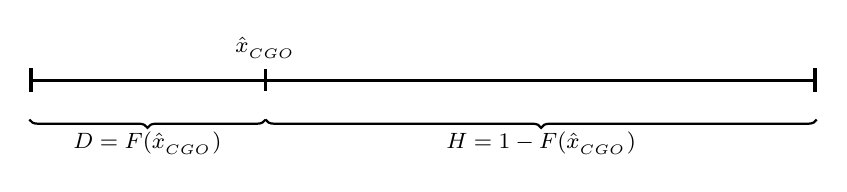
\begin{tikzpicture}[y=1cm, x=1cm, thick, font=\footnotesize]    
% axis
\draw[line width=1.2pt, |-|, >=latex'](0,0) -- coordinate (x axis) (10,0);       
\draw (3,-4pt) coordinate (t_k)          -- (3,4pt) node[anchor=south] {$\hat{x}_{_{CGO}}$};
% curly braces
\draw[decorate,decoration={brace,amplitude=3pt,mirror}] 
    (0,-0.5) coordinate (t_k_unten) -- (3,-0.5) coordinate (t_k_opt_unten); 
\node at (1.5,-0.8){$D=F(\hat{x}_{_{CGO}})$};
\draw[decorate,decoration={brace,amplitude=3pt,mirror}] 
    (3,-0.5) coordinate (t_k_unten) -- (10,-0.5) coordinate (t_k_opt_unten); 
\node at (6.5,-0.8){$H=1-F(\hat{x}_{_{CGO}})$};
\end{tikzpicture}

\item We can solve for the cutoff point:
\begin{equation}
\hat{x}_{_{CGO}}= k-d + \highlight{(d-\mu)} F(\hat{x}_{_{CGO}}). \label{eq:cgo}
\end{equation}


\end{itemize}
}

\frame
{
\frametitle{Social welfare}
\begin{itemize}
\item \emph{strategic complements} game: first mover that sets the stage 
\item If first player plays $D$, there is an incentive for the second player to follow suit 

\item Sequential game can help improve social welfare!

\item Park and Rabanal (2018): unique PBNE where the first mover follows the cutoff strategy 
\begin{equation}
\sigma_i(x_i)=D \quad \text{if} \ \ x_i\leq \hat{x}_{_{CGS}} \equiv k-\mu. 
\end{equation}

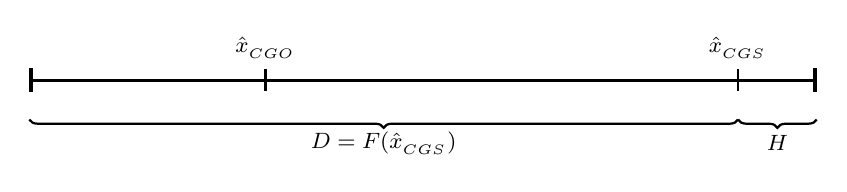
\begin{tikzpicture}[y=1cm, x=1cm, thick, font=\footnotesize]    
% axis
\draw[line width=1.2pt, |-|, >=latex'](0,0) -- coordinate (x axis) (10,0);       
\draw (3,-4pt) coordinate (t_k)          -- (3,4pt) node[anchor=south] {$\hat{x}_{_{CGO}}$};
\draw (9,-4pt) coordinate (t_k)          -- (9,4pt) node[anchor=south] {$\hat{x}_{_{CGS}}$};
% curly braces
\draw[decorate,decoration={brace,amplitude=3pt,mirror}] 
    (0,-0.5) coordinate (t_k_unten) -- (9,-0.5) coordinate (t_k_opt_unten); 
\node at (4.5,-0.8){$D=F(\hat{x}_{_{CGS}})$};
\draw[decorate,decoration={brace,amplitude=3pt,mirror}] 
    (9.0,-0.5) coordinate (t_k_unten) -- (10,-0.5) coordinate (t_k_opt_unten); 
\node at (9.5,-0.8){$H$};
\end{tikzpicture}
\end{itemize}
}

\frame
{
\frametitle{Endogenous order of play}

\begin{itemize}
\item The game proceeds as follows:
\begin{itemize}
\item \textbf{Stage 0:} Each player $i$ observes own type $x_i$, but not the other player's type $x_j$, where $j\neq i$.

\item \textbf{Stage 1:} Both players simultaneously and publicly announce a period $t_{i}\in\{1,2\}$, in which they will play

\item \textbf{Stage 2:} Each player plays $s\in\{H,D\}$ in the announced periods
\end{itemize}
     \item Because the game has strategic complements, players with a high value of $x$ should wait and play in period 2, while the players with low value of $x$ should go first and play $D$ 
     \item Cutoff strategy does not change: $\hat{x}_{_{CGE}}=\hat{x}_{_{CGS}}$.
\end{itemize}
 }
 
 
 
\frame
{
\frametitle{Predictions}

\begin{enumerate}


\item In the simultaneous conflict game  subjects play at or above the cutoff strategy $\hat{x}_{_{CGO}}$.

\item In the sequential CGS game, the first mover will increase the cutoff strategy by $\hat{x}_{_{CGS}}-\hat{x}_{_{CGO}}>0$.

\item In the endogenous CGE game, the first mover will increase the cutoff strategy by $\hat{x}_{_{CGE}}-\hat{x}_{_{CGO}}>0$.

\item The probability of observing a $DD$ outcome is greater in the CGS and CGE games compared to the CGO game by $F(\hat{x}_{_{CGS}})\cdot F(\hat{x}_{_{CGS}})-F(\hat{x}_{_{CGO}})\cdot F(\hat{x}_{_{CGO}})>0$.

\item Females will play $H$ more often compared to males in CGE due to strategic uncertainty.

\end{enumerate}

}

\frame
{
\frametitle{Procedures}
\begin{itemize}
\item Subjects recruited from Universidad del Rosario, Bogota, Colombia (ORSEE)
\item Show-up fee: COL 10K $\approx$ \$ 3.3
\item A between design, veiled gender, perfect stranger matching
\item 3 treatments: CGO, GGS and GGE
\item Each session: 
\begin{itemize}
    \item two silos
    \item 12 Ss in each silo 
    \item (almost) balance gender composition within silo
    \item each silo runs a different treatment 
\end{itemize}
\item oTree user-interface 

\end{itemize}
}



\frame
{
\frametitle{Procedures (cont'd)}
\begin{itemize}
\item Parameters 
\begin{equation}
\begin{pmatrix}
x_i\sim U[0,100] & 10+x_i \\
100-95 & 100 
\label{t:payoffreal}
\end{pmatrix}.
\end{equation}


\item Each treatment proceeds as follows
\begin{itemize}
\item 4 \emph{solo} practice rounds, where the counterparty is a robot \emph{Nash}.
\item Directly ask for the cutoff strategy: \textit{Select the min. number $\in[0,101]$ for which you will play $H$ (A) }
\end{itemize}
\end{itemize}

\begin{center}
\begin{tabular}{cc}
    0 $\rightarrow$& Always $H$ \\
    101 $\rightarrow$& Always $D$
\end{tabular}
    
\end{center}
}


\frame	
{
\frametitle{Cutoff User-Interface }
\begin{figure}[here]
\begin{center}
\includegraphics[scale=.35]{cutoffscreen.png}
%\caption{User-Interface CM treatment}
\label{fig:usercutoff}
\par\end{center}
\end{figure} 
}

\frame
{
\frametitle{Procedures Summary}

\begin{center}
\begin{tabular}{l|m{3cm}|m{3cm}|m{3cm}}
  \hline
  Step & CGO & CGS & CGE\\
  \hline \hline
I & cutoff & cutoff & cutoff \\
\hline
II& $x_i$ is revealed; H if $\mtext{cutoff}\leq x_i$ & $x_i$ is revealed; H if $\mtext{cutoff}\leq x_i$ for 1st mover (randomly chosen) 
& $x_i$ is revealed; choose $t=\{1,2\}$ \\
\hline
III & - & 2nd mover picks \textbf{s} & 2nd mover ($t=2$) picks \textbf{s} if other chose $t=1$. \\

\end{tabular}
\begin{itemize}
\item CGE has additional strategic uncertainty ($t$): if both Ss pick same $t$, then they play a simultaneous game
\end{itemize}
\end{center}

}

\frame
{
\frametitle{Summary of results (pooled data)}
\begin{center}
\begin{figure}[ht]
\centering{}%
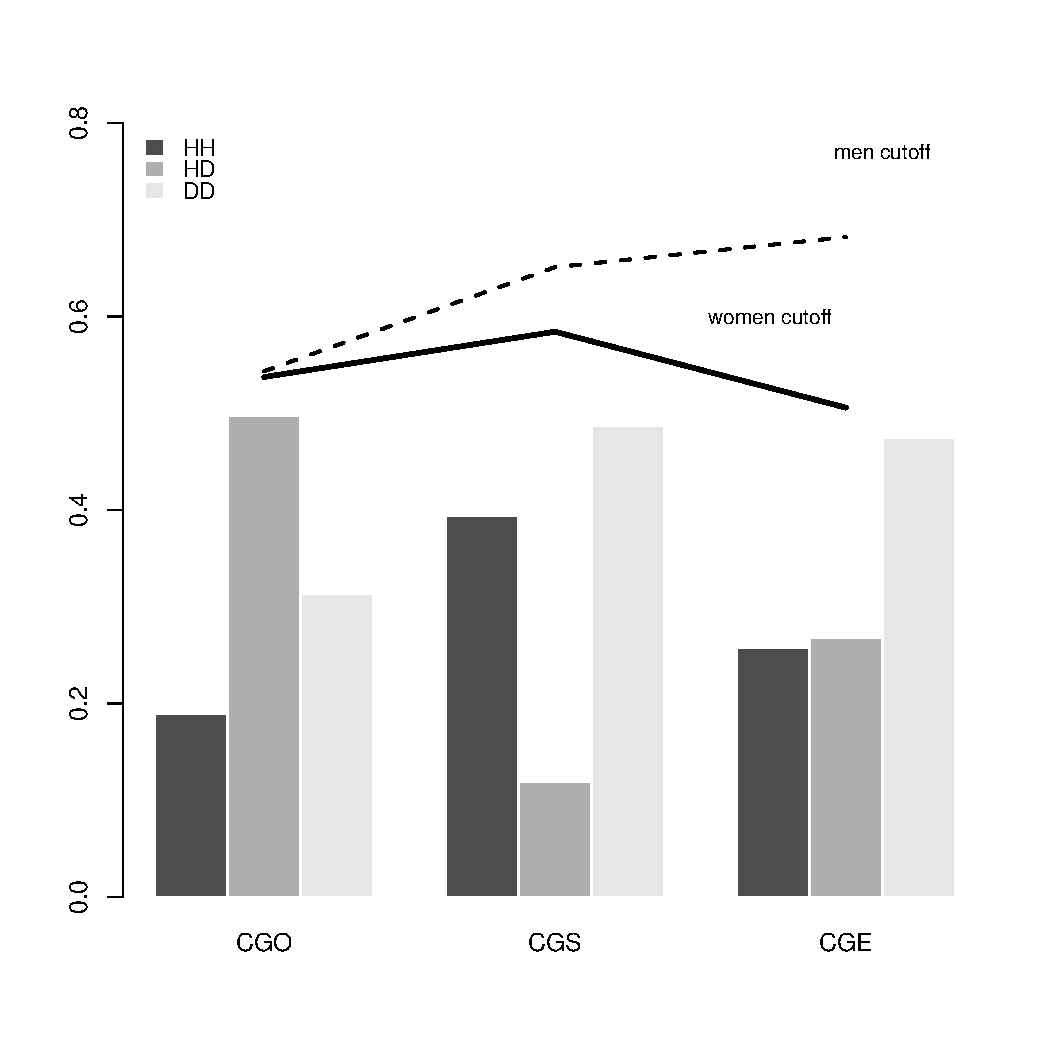
\includegraphics[scale=0.5]{jointcut.pdf}%
%\caption{CDF of $x$ by subject in CM and DM. Each observation is based on the median subject choice for periods 26-50. The vertical lines represent the predicted equilibrium under DM and CM. }
\label{fig:jointcut}
\end{figure}
\par\end{center}
}

\frame
{
\frametitle{CGE (pooled data)}
\begin{center}
\begin{figure}[ht]
\centering{}%
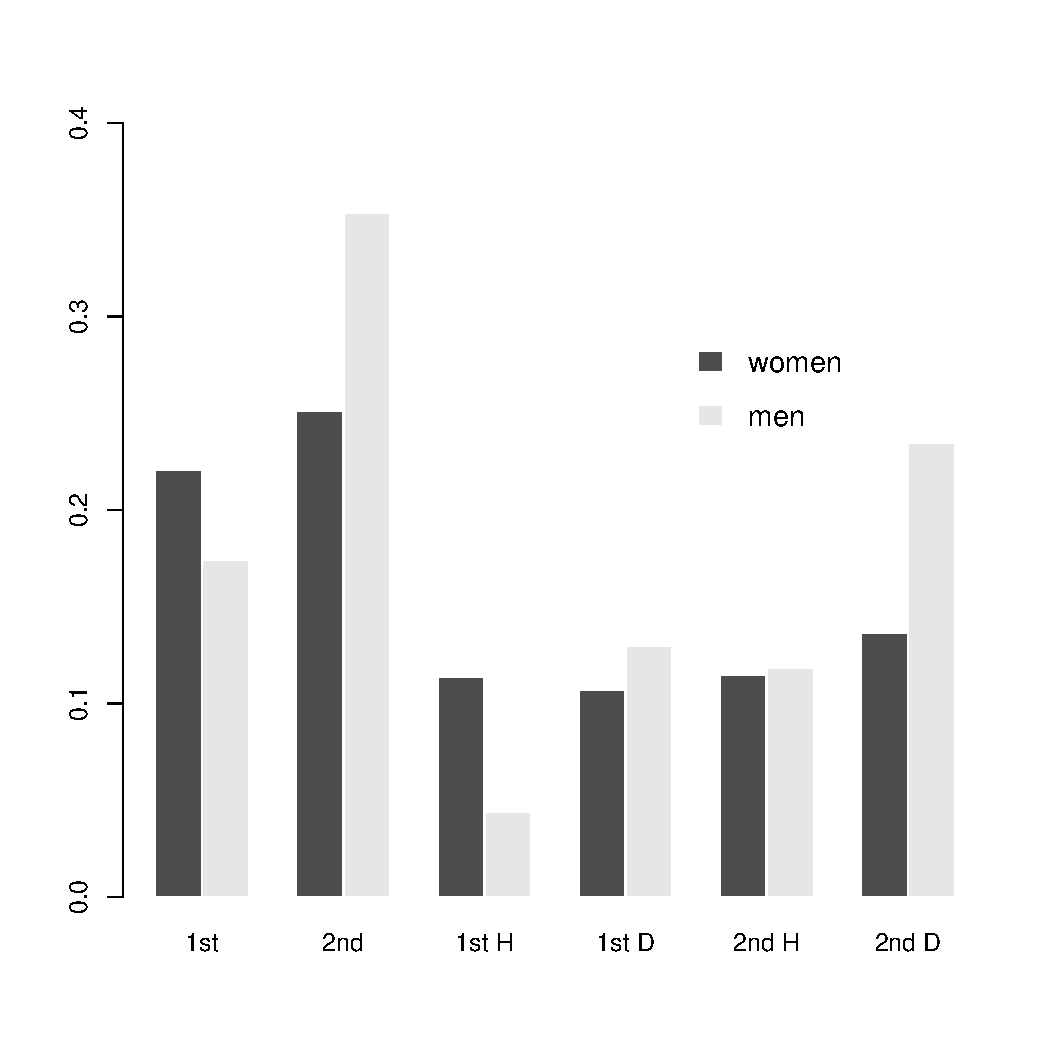
\includegraphics[scale=0.5]{countgendermoveplay.pdf}%
%\caption{CDF of $x$ by subject in CM and DM. Each observation is based on the median subject choice for periods 26-50. The vertical lines represent the predicted equilibrium under DM and CM. }
\label{fig:jointcut}
\end{figure}
\par\end{center}
}




\frame	
{
\frametitle{CGE (pooled data)}
\begin{table}[ht]
\centering
\footnotesize
\begin{tabular}{l|ccc}
    & one-shot $t=1$  & seq. & one-shot $t=2$\\
    \hline
  HH    &    2.31 &17.59  &      3.24\\
  HD    &    6.48 & 3.70 &      15.28\\
  DD     &   5.09 &34.72&       11.57
\end{tabular}
\label{table1}
\caption{CGE. Frequency of cells and timing (\%) }

\end{table}
}

\frame
{
\frametitle{Subject data}
\begin{center}
\begin{figure}[ht]
\centering{}%
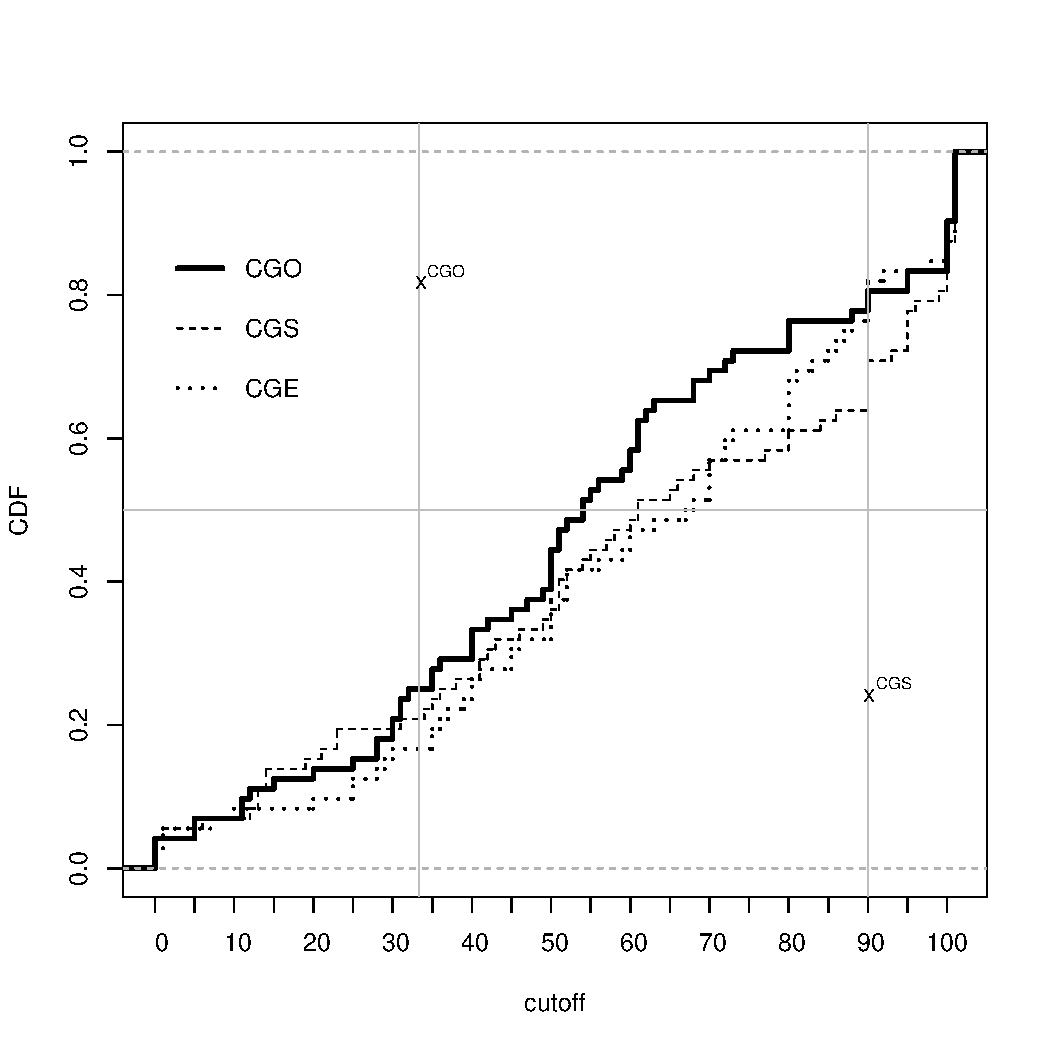
\includegraphics[scale=0.5]{cdfcutoff.pdf}%
%\caption{CDF of $x$ by subject in CM and DM. Each observation is based on the median subject choice for periods 26-50. The vertical lines represent the predicted equilibrium under DM and CM. }
\label{fig:allcdfsubj}
\end{figure}
\par\end{center}
}

\frame
{
\frametitle{Subject data - female}
\begin{center}
\begin{figure}[ht]
\centering{}%
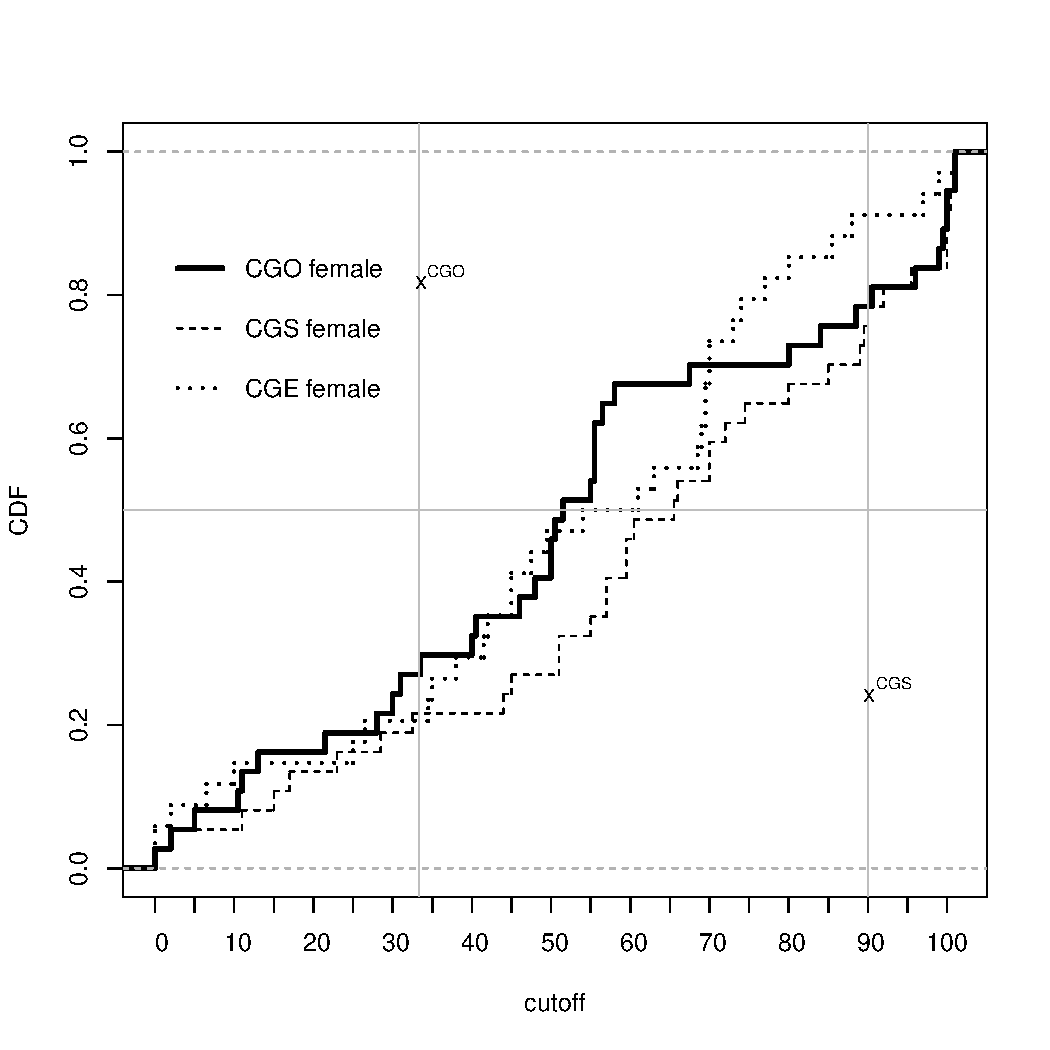
\includegraphics[scale=0.5]{cdfcutoffgender_female.pdf}%
%\caption{CDF of $x$ by subject in CM and DM. Each observation is based on the median subject choice for periods 26-50. The vertical lines represent the predicted equilibrium under DM and CM. }
\label{fig:fecdfsubj}
\end{figure}
\par\end{center}
}

\frame
{
\frametitle{Subject data - male}
\begin{center}
\begin{figure}[ht]
\centering{}%
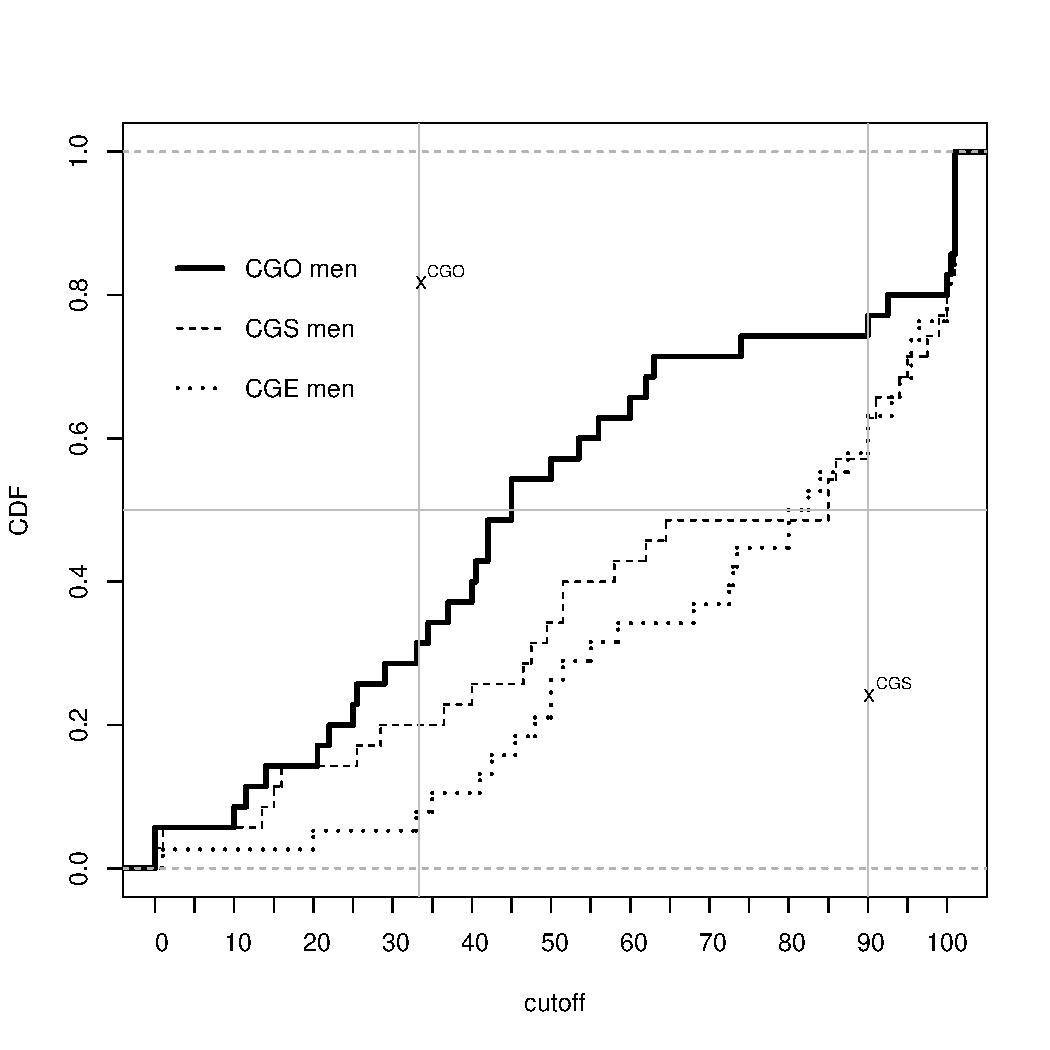
\includegraphics[scale=0.5]{cdfcutoffgender_male.pdf}%
%\caption{CDF of $x$ by subject in CM and DM. Each observation is based on the median subject choice for periods 26-50. The vertical lines represent the predicted equilibrium under DM and CM. }
\label{fig:fecdfsubj}
\end{figure}
\par\end{center}
}

\frame
{
\frametitle{Subject data - CGO}
\begin{center}
\begin{figure}[ht]
\centering{}%
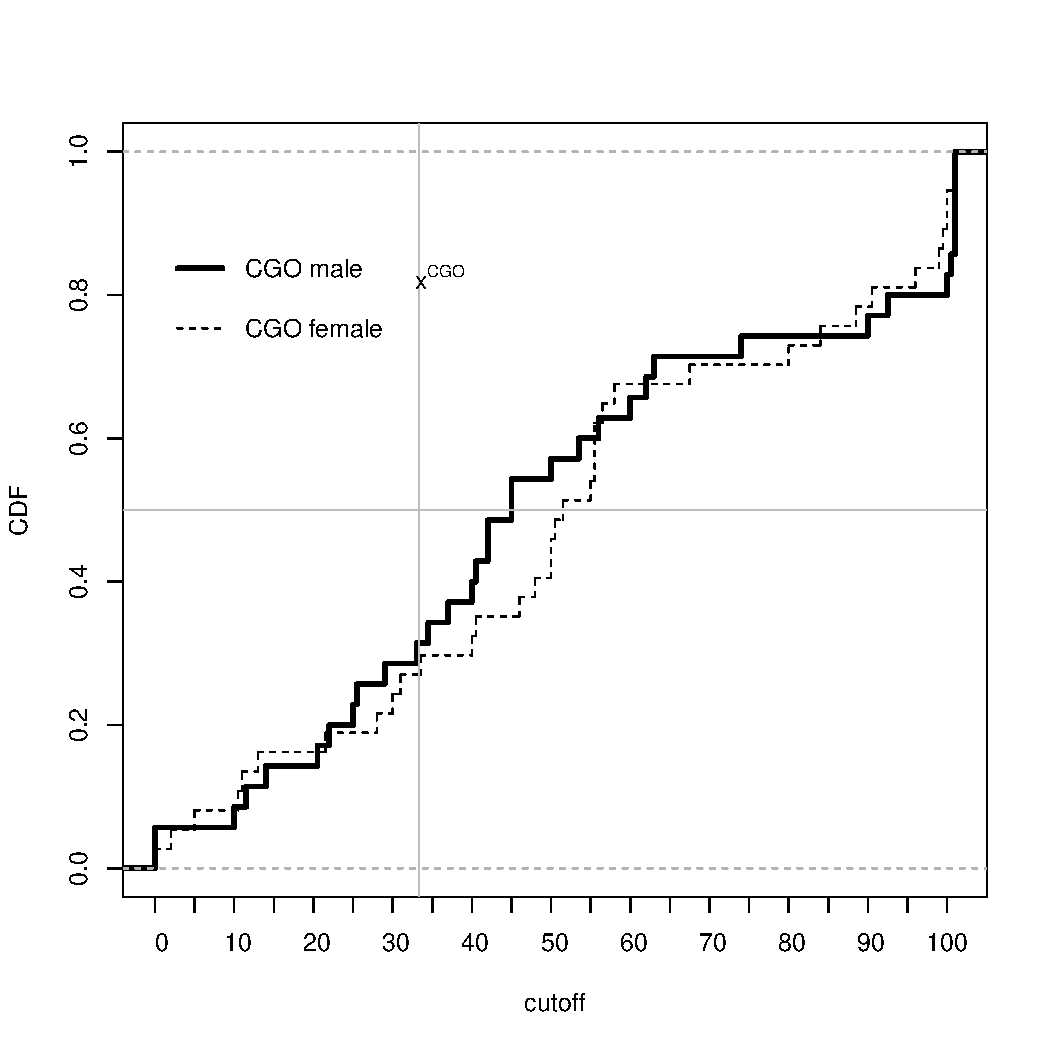
\includegraphics[scale=0.5]{cdfcutoffgender_o.pdf}%
%\caption{CDF of $x$ by subject in CM and DM. Each observation is based on the median subject choice for periods 26-50. The vertical lines represent the predicted equilibrium under DM and CM. }
\label{fig:onecdfsubj}
\end{figure}
\par\end{center}
}

\frame
{
\frametitle{Subject data - CGS}
\begin{center}
\begin{figure}[ht]
\centering{}%
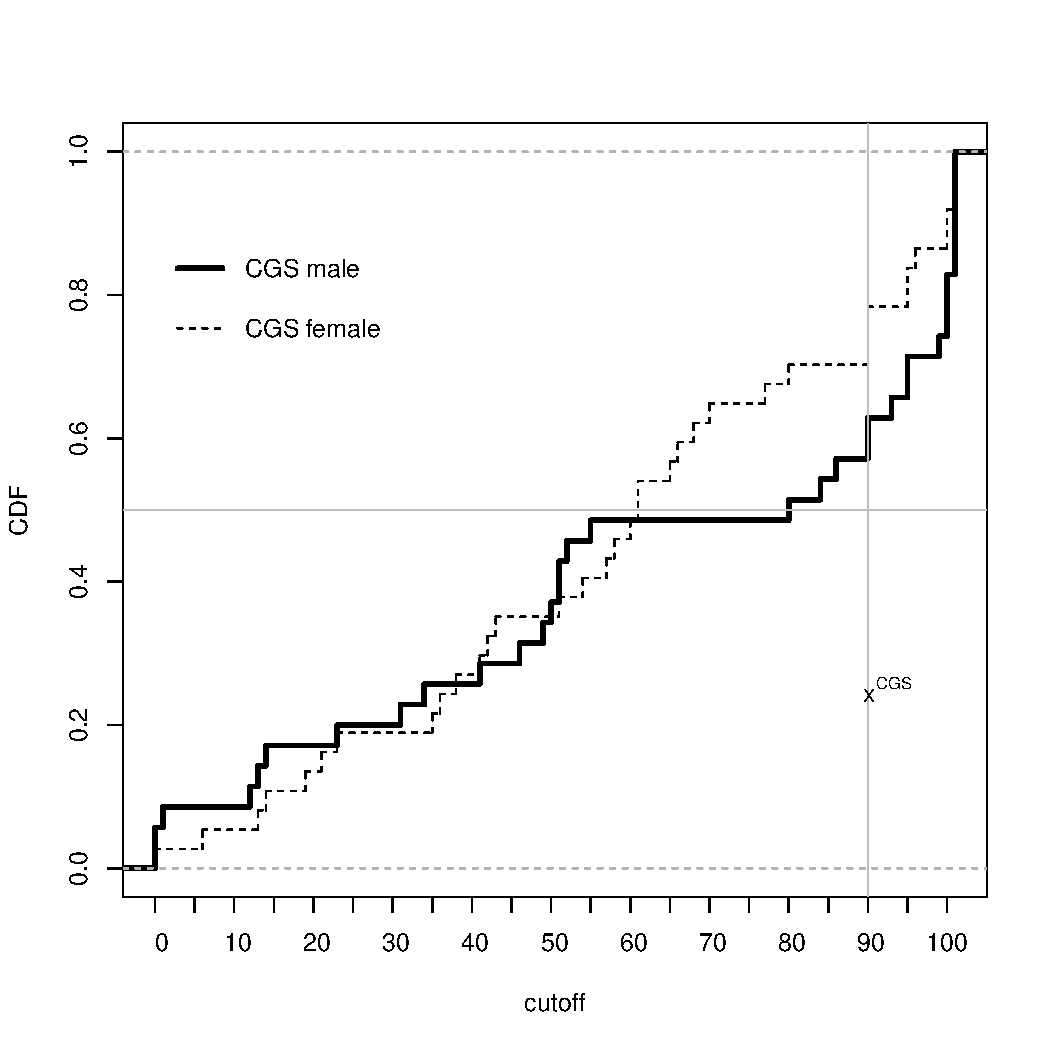
\includegraphics[scale=0.5]{cdfcutoffgender_s.pdf}%
%\caption{CDF of $x$ by subject in CM and DM. Each observation is based on the median subject choice for periods 26-50. The vertical lines represent the predicted equilibrium under DM and CM. }
\label{fig:sscdfsubj}
\end{figure}
\par\end{center}
}

\frame
{
\frametitle{Subject data - CGE}
\begin{center}
\begin{figure}[ht]
\centering{}%
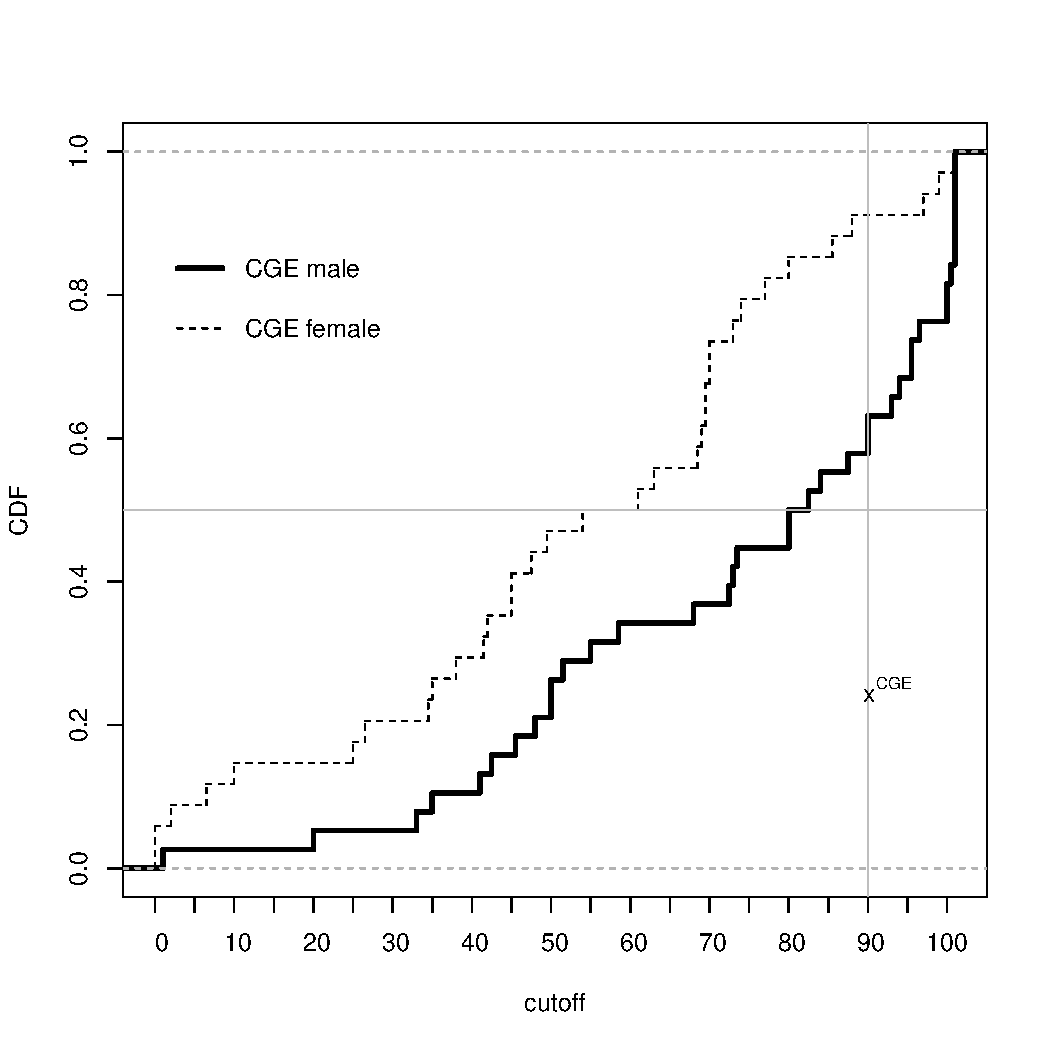
\includegraphics[scale=0.5]{cdfcutoffgender_e.pdf}%
%\caption{CDF of $x$ by subject in CM and DM. Each observation is based on the median subject choice for periods 26-50. The vertical lines represent the predicted equilibrium under DM and CM. }
\label{fig:eecdfsubj}
\end{figure}
\par\end{center}
}

\frame
{
\frametitle{Conclusion}
\begin{itemize}
\item Sequential moves improves social welfare 
\item Strategic uncertainty about the timing of the game deters females from playing $D$
\item Future applications: bank runs, population games
\end{itemize}
}


\end{document}

